% !TEX encoding = UTF-8
% !TEX TS-program = pdflatex
% !TEX root = ../tesi.tex

\newpage
\section{Progettazione}
\label{sec:progettazione}

\subsection{Package it.imolinfo.apat}\label{subsec:package}
Questo è il root package del tool, contiene altri package e le due classi elencate successivamente.
\begin{namespacedesc}
    \classdesc{ApatLauncher}{è la classe di launcher del tool, si occupa principalmente di mettere in relazione di observed-observer i componenti della vista con i dati del modello;}
    \classdesc{Utils}{la classe di utilities che ha delle funzioni statiche utilizzate nel tool per evitare la ripetizione del codice.}
\end{namespacedesc}

\subsection{Package it.imolinfo.apat.controller}\label{subsec:package-it.imolinfo.apat.controller} %**************************
Questo è il package che contiene la classe Controller e ciò che riguarda l'interazione del controller con il filesystem.
\begin{figure}[H]
    \centering
    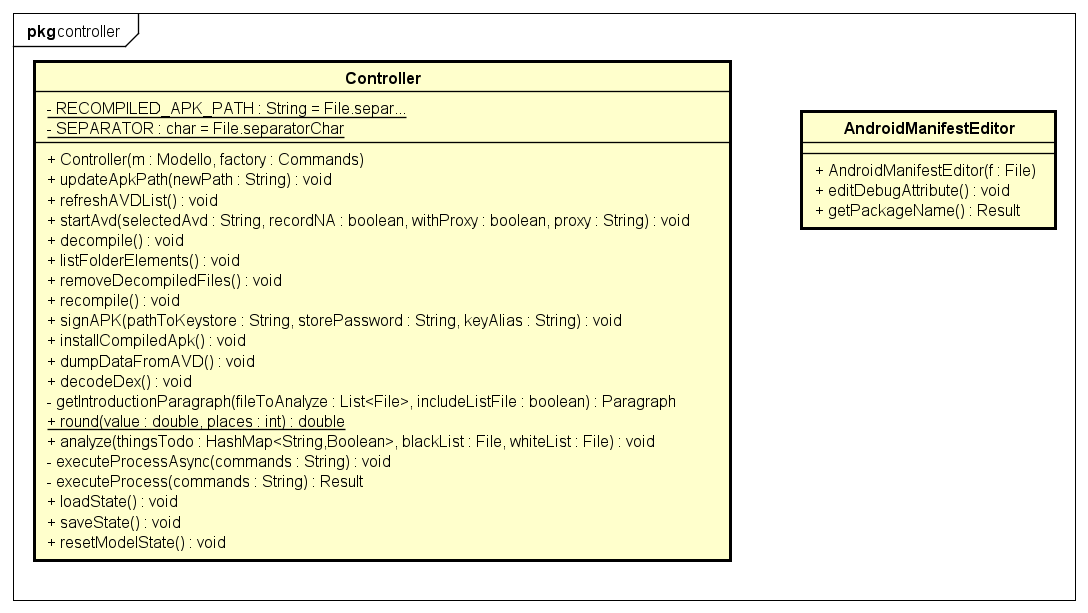
\includegraphics[width=14cm,height=8cm]{./immagini/diagrammi_uml/controller.png}
    \caption{Package Controller.}\label{fig:controller_diagram}
\end{figure}
\begin{namespacedesc}
    \classdesc{AndroidManifestEditor.java}{è la classe che si occupa, dato un file di tipo AndroidManifest, di modificare e/o aggiungere il tag \textit{debuggable} impostando il suo valore a \textit{true};}
    \classdesc{Controller}{è il controller del MVC, si occupa di effettuare le operazioni di decompilazione, ricompilazione, decodifica e analisi dei file;}
\end{namespacedesc}

\subsection{Package it.imolinfo.apat.model}\label{subsec:package-it.imolinfo.apat.model} %**************************
Questo package contiene le classi che riguardano il modello del pattern Model View Controller.
\begin{figure}[H]
    \centering
    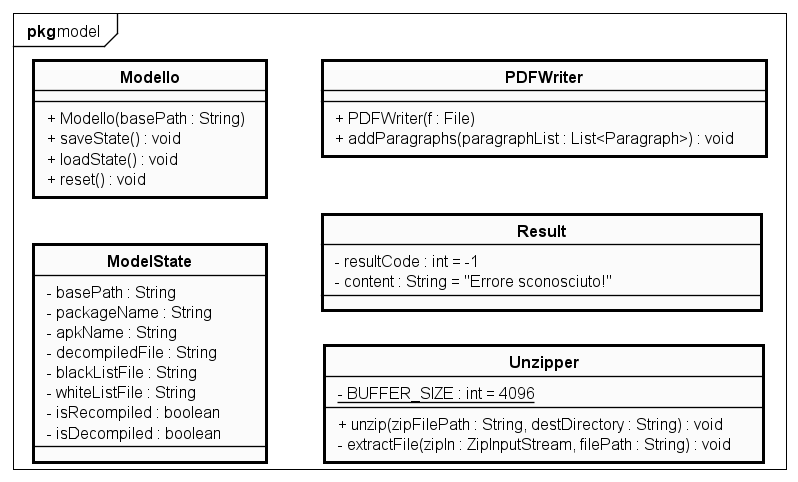
\includegraphics[width=14cm,height=8cm]{./immagini/diagrammi_uml/model.png}
    \caption{Package Model.}\label{fig:model_diagram}
\end{figure}
\begin{namespacedesc}
    \classdesc{Modello}{la classe che contiene i dati utili al corretto funzionamento del tool;}
    \classdesc{ModelState}{è la classe che viene usata per poter salvare lo stato del funzionamento del tool. Lo stato viene salvato quando viene chiuso il tool, e viene ricaricato al successivo avvio;}
    \classdesc{PDFWriter}{è la classe wrapper che si occupa della creazione del file PDF per salvare i risultati dell'analisi;}
    \classdesc{Result}{è la classe di messaggio che viene restituita quando il tool interagisce con il file system;}
    \classdesc{Unzipper}{è la classe si occupa di decomprimere i file .zip;}
    \classdesc{Dumper}{è la classe che si occupa di effettuare il dump dei dati da un file con estensione \textit{db};}
\end{namespacedesc}

\subsection{Package it.imolinfo.apat.pattern}\label{subsec:package-it.imolinfo.apat.pattern} %**************************
Questo package contiene dei sotto-package ognuno dei quali rappresenta un design pattern utilizzato nello sviluppo del tool.\\
Il package analyzer è composto dalle seguenti classi:

\begin{namespacedesc}
    \classdesc{analyzer.Analyze}{è l'interfaccia di base del pattern Decorator.}
    \classdesc{analyzer.BaseAnalyzer}{è la classe dell'oggetto base che viene decorato.}
    \classdesc{analyzer.BaseAnalyzeDecorator}{è la classe astratta del decorator di base che implementa l'interfaccia Analyze, e ha un metodo astratto \textit{doAnalysis()} che deve essere implementato dai decorator concreti.}
    \classdesc{analyzer.DumpDataBase}{è il decorator che si occupa di estrarre i contenuti dei file \textit{.db} scaricati dall'area di storage dell'app.}
    \classdesc{analyzer.DumpedFilesAnalyzer}{è il decorator che si occupa di analizzare i file dell'area di storage dell'applicazione con estensione \textit{XML} e \textit{JSON}. Principalmente, legge il contenuto di tali file, e in base ad una whitelist, seleziona quali risultati restituire al chiamante.}
    \classdesc{analyzer.LambdaCounter}{è il decorator che conta il numero di lambda presenti per ogni classe di codice \textit{.java} decompilato.}
    \classdesc{analyzer.StringFinder}{è il decorator che analizza i file di tipo \textit{.java}, ed estrae le stringhe hardcoded, può essere utilizzato insieme a un blacklist delle stringhe che devono essere ignorate.}
\end{namespacedesc}
Il package observer è composto da seguenti classi:
\begin{namespacedesc}
    \classdesc{observer.Observable}{la classe parametrizzata T che può essere osservata;}
    \classdesc{observer.Observer}{l'interfaccia parametrizzata che ha il ruolo dell'observer;}
\end{namespacedesc}
Il package factory method è composto da seguenti classi:
\begin{namespacedesc}
    \classdesc{cliCommandFactory.Commands}{è l'interfaccia che contiene i metodi, dove ognuno dei quali deve generare delle istruzioni per la linea di comando.}
    \classdesc{cliCommandFactory.CommandFactory}{è la classe astratta che implementa la precedente interfaccia, con un costruttore di default che richiede un path di base.}
    \classdesc{cliCommandFactory.UnixCommandFactory}{è l'implementazione della classe astratta CommandFactory per il sistema UNIX.}
    \classdesc{cliCommandFactory.WindowsCommandFactory}{è l'implementazione della classe astratta CommandFactory per il sistema Windows.}
\end{namespacedesc}

\subsection{Package it.imolinfo.apat.view}\label{subsec:package-it.imolinfo.apat.view} %**************************
\begin{figure}[H]
    \centering
    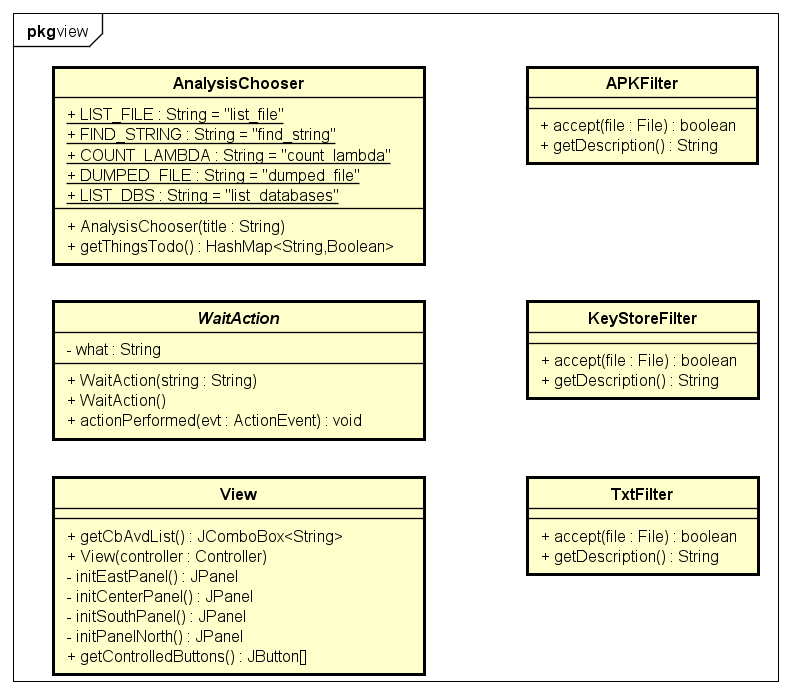
\includegraphics[width=14cm,height=10cm]{./immagini/diagrammi_uml/view.png}
    \caption{Package View.}\label{fig:view_diagram}
\end{figure}
\begin{namespacedesc}
    \classdesc{AnalysisChooser}{è la finestra che mostra le opzioni di analisi.}
    \classdesc{View}{è la finestra principale, dove permette di selezionare il file \textit{apk} da decompilare ed analizzare.}
    \classdesc{WaitAction}{è una classe astratta che a sua volta eredita dalla classe Action e permette di eseguire un processo mostrando la barra del caricamento.}
    \classdesc{ApkFilter}{è l'implementazione dell'interfaccia \textbf{FileFilter} che accetta solo i file di tipo \textit{APK}.}
    \classdesc{KeyStoreFilter}{è l'implementazione dell'interfaccia \textbf{FileFilter} che accetta solo i file di tipo \textit{JKS}.}
    \classdesc{TextFilter}{è l'implementazione dell'interfaccia \textbf{FileFilter} che accetta solo i file di tipo \textit{txt}.}
\end{namespacedesc}